% Template for MEng/BEng/MSc final reports
% EEE Department - Imperial College London
%
% INSTRUCTIONS
% (1) Compile using LuaLatex (it is the successor of pdflatex). To check this on Overleaf, click on the Menu on the top left.
% (2) Complete the SETUP below
% (3) Students of Imperial College can claim a free premium Overleaf account, see https://www.imperial.ac.uk/admin-services/ict/self-service/computers-printing/devices-and-software/get-software/get-software-for-students/overleaf/ 
% Claim the free premium account because as your report becomes more and more complex you may reach the timeout limit of the free account.

%%%%%%%%%%%%%%%%%%%%%%%%%%%%%%%%%%%%%%%
% DO NOT MODIFY FROM HERE ...
\documentclass[10pt]{ic_eee_thesis}

\usepackage[style=ieee,backend=biber,hyperref=auto]{biblatex}
\addbibresource{references.bib}
% ... TO HERE
%%%%%%%%%%%%%%%%%%%%%%%%%%%%%%%%%%%%%%%


%%%%%%%%%%%%%%%% SETUP %%%%%%%%%%%%%%%%
%%%%%%%%%%%%%%%%%%%%%%%%%%%%%%%%%%%%%%%
% EDIT THE FOLLOWING INFORMATION WITH YOUR DATA
% COMPLETE PART A
% IF YOU ARE DOING A MENG/BENG COMPLETE ALSO PART B
% IF YOU ARE DOING AN MSC IGNORE PART B
% LINES STARTING WITH % ARE COMMENTS. UNCOMMENT JUST ONE OF A SET OF OPTIONS
% MAKE SURE YOU CHECK AND UPDATE ALL INFORMATION, INCLUDING SUBMITYEAR


%%%%%%%%%%% PART A %%%%%%%%%%%
% PICK A DEGREE FROM THE LIST BELOW 
% BY COMMENTING OUT/IN YOUR DEGREE
% DO NOT MODIFY THE NAMES
%\degree{MEng}
%\degree{BEng}
\degree{MSc}

\title{Title of your FYP/MSc Report}
\subtitle{Subtitle if needed} % use \subtitle{} to remove the subtitle
\author{N.S. Surname}
\cid{00000000}
\supervisor{Dr N.S. Surname \\[1mm] Prof. A. Another} %UK: Dr no dot, prof has dot
\submityear{2024}

% PICK A COURSE FROM THE LIST BELOW 
% DO NOT MODIFY THE NAMES
%%%%%%%%% BENG-MENG COMMON LIST
%\course{Electrical and Electronic Engineering}
%\course{Electronic and Information Engineering}
%%%%%%%%% MENG-ONLY LIST
%\course{Electrical and Electronic Engineering with Management} 
%\course{Electrical and Electronic Engineering with a Year Abroad}
%\course{Electronic and Information Engineering with a Year Abroad}
%%%%%%%%% MSC LIST
%\course{Analogue and Digital Integrated Circuit Design}
%\course{Applied Machine Learning}
%\course{Communications and Signal Processing}
\course{Control and Optimisation}
%\course{Future Power Networks}


% Do you want a list of figures?
% Do you want a list of tables?
% Do you want an acknowledgement page?
% Do you want a list of acronyms?
\setboolean{list_of_figures}{true} % false or true - Default is true
\setboolean{list_of_tables}{false} % false or true - Default is false
\setboolean{acknowledgement}{true} % false or true - Default is true
\setboolean{acronyms}{true} % false or true - Default is true

% If you want to print your thesis, consider changing the command below to true. If true, the command adds labels at the edge of the pages which will make easy to identify a chapter running through the pages with the finger. It is just a visual setting. The default values are different for MENG/BEng and MSc as a consequence of the different approval process. In any case, you can change this to either true or false as you prefer.
%\setboolean{edge_labels}{false} % default for MEng
\setboolean{edge_labels}{true} % default for MSc

%The preferred spacing for FYP/MSc reports is doublespacing. This is because it is easier for markers to annotate the document while marking. Some students requested the implementation of the singlespacing option. This can be activated below by changing from true to false, but discuss this with your supervisor first.
\setboolean{double_spacing}{true} %Default is true. If you want to change this, ask your supervisor if they are OK with singlespacing.

%%%%%%%%%%% PART B %%%%%%%%%%% 
% ONLY FOR MENG/BENG. MSC IGNORE THIS
% THESE ADDITIONAL SETTINGS HAVE BEEN ASKED BY THE MEng COMMITTEE BUT NOT BY THE MSC COMMITTEE
% Is this an interim report or final thesis?
\setboolean{final_thesis}{true} % true for final Thesis / false for interim report
\secondmarker{Second Marker\\[2mm]{\large \textsc Dr Jane Doe}} %If you do not know who your second marker is, use \secondmarker{}

%%%%%%%%%%%%% END SETUP %%%%%%%%%%%%%%%
%%%%%%%%%%%%%%%%%%%%%%%%%%%%%%%%%%%%%%%


% ADDITIONAL PACKAGES
% You can add your packages below. Note that the following packages are already loaded: pgfcore, geometry, bookmark, graphicx, setspace, kantlipsum, fontspec, polygrossia (default English), minitoc, silence, background, xpatch, tikzpagenodes, totcount, fancyhdr, titlesec and the tikz libraries calc, shapes.symbols and shapes.misc  

%Examples
\usepackage{amsmath}
\usepackage{amsfonts} 
%...

% ADDITIONAL COMMANDS
%Examples
\DeclareMathOperator{\diag}{diag}
\DeclareMathOperator{\vect}{vec}
%...


\begin{document}

\preamble % Do not change - required

% EDIT THE CONTENT OF THE FILES
% Abstract.tex
% OrigSta_Copyright.tex
% Acknowledgement.tex
% You can find them under the folder 
% "chapters" on the left column

% ADD AS MANY CHAPTERS AS NEEDED
% BY CREATING .TEX FILES IN THE FOLDER chapters
% AND ADDING \input{namechapter.tex} BELOW
\doublespacing % Do not change - required

\chapter{Introduction}
\label{ch1}

%%%%%%%%%%%%%%%%%%%%%%%%%%%%%%%%%%%%%%%
% IMPORTANT
\begin{spacing}{1} %THESE FOUR
\minitoc % LINES MUST APPEAR IN
\end{spacing} % EVERY
\thesisspacing % CHAPTER
% COPY THEM IN ANY NEW CHAPTER
%%%%%%%%%%%%%%%%%%%%%%%%%%%%%%%%%%%%%%%


\section{Title section}

\kant[1]

Example of citation are here
\cite{AdaAroKre:71,PadScaAst:16a,PadScaAst:16b,PavVdWNij:06,PurBorVar:96,SLICOT,Sca:16,Sca:16a,Sca:16b,Sca:17,Sca:18}.

And some acronyms: \ac{USA} and \ac{LTI} systems.

\subsection{Title subsection}

\kant[1-10]


\begin{figure}
\centering
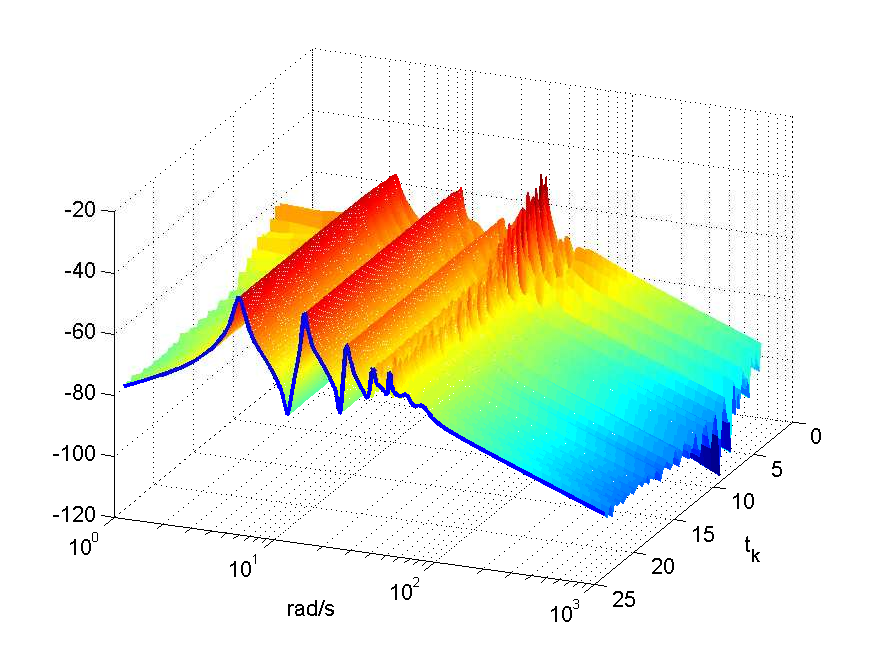
\includegraphics[width=0.8\columnwidth]{imgs/buildmagnitude.pdf}
\caption[Short description for list of figures]{This figure is taken from \cite{Sca:16}.}
\label{fig-magnitude}
\end{figure}%


\kant[1-4]

\subsection{Title subsection}

\kant[1-3]


\section{Title section}

\kant[1-5]

\section{Notation}

Standard notation has been adopted in the Thesis, most of which is defined in this section and used throughout the remainder of the Thesis. When new notation, not included in this section is introduced, this is defined in the relevant parts of the Thesis.\smallskip\\
\indent The symbol $\mathbb{R}_{\ge0}$ ($\mathbb{R}_{>0}$) denotes the set of non-negative (positive) real numbers; $\mathbb{C}_{<0}$ denotes the set of complex numbers with strictly negative real part; $\mathbb{C}_{0}$ denotes the set of complex numbers with zero real part and $\mathbb{D}_{<1}$ the set of complex numbers with modulo less than one.\smallskip\\
\indent The symbol $I$ denotes the identity matrix and $\sigma(A)$ denotes the spectrum of the matrix $A\in\mathbb{R}^{n\times n}$. The symbol $\otimes$ indicates the Kronecker product and $||A||$ indicates the induced Euclidean matrix norm. Given a list of $n$ elements $a_i$, $\diag(a_i)$ indicates a diagonal matrix with diagonal elements equal to the $a_i$'s. The vectorization of a matrix $A\in\mathbb{R}^{n\times m}$, denoted by $\vect(A)$, is the $nm \times 1$ vector obtained by stacking the columns of the matrix $A$ one on top of the other, namely $\vect(A)=[a_1^{\top},a_2^{\top},\dots,a_m^{\top}]^{\top}$, where $a_i\in\mathbb{R}^n$ are the columns of $A$ and the superscript $\top$ denotes the transposition operator. The superscript $*$ indicates the conjugate transpose operator.\smallskip\\
\indent The symbol $\Re[z]$ indicates the real part of the complex number $z$, $\Im[z]$ denotes its imaginary part and $\iota$ denotes the imaginary unit. The symbol $\epsilon_k$ indicates a vector with the $k$-th element equal to 1 and with all the other elements equal to 0. Given a function $f$, $\overline{F}$ represents its phasor at $\omega$, whereas $<\!f(t)\!>$ indicates its time average.\smallskip\\
\indent Given a set of delays $\{\tau_j\}$, the symbol $\mathfrak{R}_T^n=\mathfrak{R}_T^n([-T,0],\mathbb{R}^n)$, with $T=  \max_j\{\tau_j\}$, indicates the set of continuous functions mapping the interval $[-T,0]$ into $\mathbb{R}^n$ with the topology of uniform convergence . The subscripts ``$\tau_j$'' and ``$\chi_j$'' denote the translation operator, \textit{e.g.}\ $x_{\tau_j}(t)=x(t-\tau_j)$.\smallskip\\
\indent Let $\bar s \in \mathbb{C}$ and $A(s)\in \mathbb{C}^{n \times n}$. Then $\bar s\notin\sigma(A(s))$ means that $\det(\bar s I-A(\bar s ))\ne0$. $\sigma(A(s))\subset\mathbb{C}_{<0}$ means that for all $\bar s$ such that $\det(\bar s I-A(\bar s ))=0$, $\bar s \in\mathbb{C}_{<0}$.\smallskip\\
\indent The symbol $\mathcal{L}(f(t))$ denotes the Laplace transform of the function $f(t)$ (provided that $f(t)$ is Laplace transformable) and $\mathcal{L}^{-1}\{F(s)\}$ denotes the inverse Laplace transform of $F(s)$ (provided it exists). With some abuse of notation, $\sigma(\mathcal{L}(f(t)))$ denotes the set of poles of $\mathcal{L}(f(t))$. Given two functions, $f:Y\to Z$ and $g:X\to Y$, with $f\,\circ\,g:X\to Z$ we denote the composite function $(f\,\circ\,g)(x)=f(g(x))$ which maps all $x\in X$ to $f(g(x))\in Z$.


\section{Published material}

\kant[1]

\doublespacing % Do not change - required

\chapter{Title chapter 2}
\label{ch2}

%%%%%%%%%%%%%%%%%%%%%%%%%%%%%%%%%%%%%%%
% IMPORTANT
\begin{spacing}{1} %THESE FOUR
\minitoc % LINES MUST APPEAR IN
\end{spacing} % EVERY
\thesisspacing % CHAPTER
% COPY THEM IN ANY NEW CHAPTER
%%%%%%%%%%%%%%%%%%%%%%%%%%%%%%%%%%%%%%%


\kant[1]

\section{Title section 2.1}

\kant[1-2]

\subsection{If needed}

\kant[1]

\subsection{If needed}

\kant[1]

\section{Title section 2.2}

\kant[1-2]

\subsection{If needed}

\kant[1]

\subsection{If needed}

\kant[1]

\section{Title section 2.3}

\kant[1-2]

\subsection{If needed}

\kant[1]

\subsection{If needed}

\kant[1]

% You can change the title of the conclusions by changing the text between { }
\conclusions{Conclusions} % Do not remove - required
% EDIT THE CONTENT OF THE FILE
% Conclusions.tex
% You can find it under the folder 
% "chapters" on the left column

% APPENDICES ARE OPTIONAL
% COMMENT OUT BOTH LINES BELOW TO REMOVE THEM
% ADD CHAPTERS TO ADD MULTIPLE APPENDICES
\appendix 
\doublespacing % Do not change - required

\chapter{Title of the Appendix}

\thesisspacing % Do not change - required

% Example text
\kant[1]
%\input{AppendixB.tex} % Example second appendix (need to create the file in "chapters")


\cleardoublepage % Do not change - required
\RemoveLabels % Do not change - required
\thesisspacing % Do not change - required
\printbibliography[title={Bibliography},heading=bibintoc] % Do not change - required

\end{document}
